% !TEX encoding = UTF-8 Unicode
\documentclass[9pt,pdf]{beamer}
\usepackage{graphicx}
\usepackage[T2A]{fontenc}
\usepackage[utf8]{inputenc}
\usepackage[russian]{babel}
\usepackage{tikz}
\usepackage{natbib}
\usepackage{tabularx}

\usetikzlibrary{decorations.markings}

\usetikzlibrary{decorations.pathmorphing}

\tikzset{snake it/.style={decorate, decoration=snake}}

\usetheme{Madrid}

\title{Исследование порога Оже-процессов в гетероструктурах с КЯ $Hg_x Cd_{1-x} Te$.}
\author{Выполнил: Куликов Н.С.\\
        Научный руководитель: Морозов С.В.}
\institute{ИФМ РАН}
\date{2019}

\newcolumntype{Y}{>{\centering\arraybackslash}X}

\begin{document}

  \frame{\titlepage}

  \begin{frame}
    Было получено стимулированное излучение на длинах 
    волн $\sim 30~\mu m$ в структурах HgCdTe при $T=8~K$.

    \begin{center}
      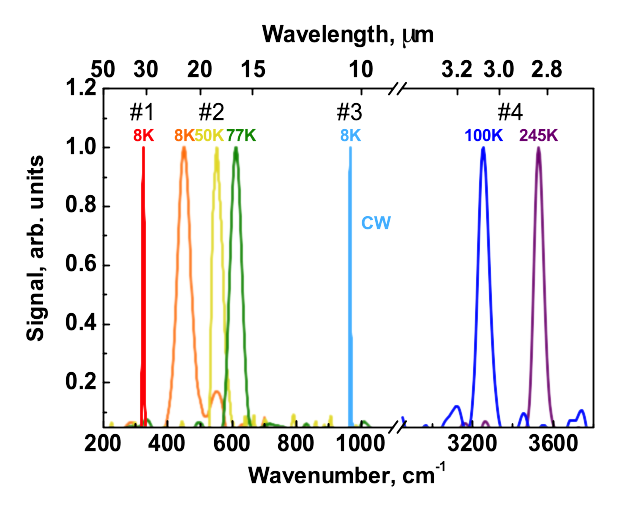
\includegraphics[width=0.75\textwidth]{images/spectre_30mum.png}
    \end{center}

    Можно ли поднять рабочую температуру?
  \end{frame}

  \begin{frame}
    \frametitle{Типы рекомбинации}
    \begin{columns}
      \column{0.33\textwidth}
        \begin{center}
          \textbf{Излучательная}

          \resizebox{0.75\textwidth}{!}{
            \begin{tikzpicture}
              \begin{scope}[very thick,decoration={
                markings,
                mark=at position 0.5 with {\arrow{>}}}
                ]
              \draw[domain=-1.3:1.3,smooth,variable=\x] plot ({\x},{0.5 * \x * \x + 0.75});
              \draw[domain=-2:2,smooth,variable=\x] plot ({\x},{-0.25 * \x * \x - 0.75});
              \draw[color=black, fill=blue] (0., 0.75) circle (.1);
              \draw[postaction={decorate}, blue, thick] (0., 0.75) -- (0., -0.75); 
              \draw[color=black, fill=red] (0., -0.75) circle (.1);
              \draw[->, snake it] (0.1, 0.) -- (1.1, 0.);
              \end{scope}
            \end{tikzpicture}
          }
          Целевой процесс - нужно только усиливать, а остальное - подавлять.

        \end{center}
      \column{0.33\textwidth}
        \begin{center}
          \textbf{Шокли-Рида-Холла (SRH)}

          \resizebox{0.75\textwidth}{!}{
            \begin{tikzpicture}
              \begin{scope}[very thick,decoration={
                markings,
                mark=at position 0.5 with {\arrow{>}}}
                ]
              \draw[domain=-1.3:1.3,smooth,variable=\x] plot ({\x},{0.5 * \x * \x + 0.75});
              \draw[domain=-2:2,smooth,variable=\x] plot ({\x},{-0.25 * \x * \x - 0.75});
              \draw (-0.5, 0.) -- (0.5, 0.);
              \draw[color=black, fill=blue] (0., 0.75) circle (.1);
              \draw[postaction={decorate}, blue, thick] (0., 0.75) -- (0., 0.); 
              \draw[color=black, fill=red] (0., -0.75) circle (.1);
              \draw[postaction={decorate}, red, thick] (0., -0.75) -- (0., 0.); 
              \end{scope}
            \end{tikzpicture}
          }
        \end{center}
        
        Происходит с участием примесей. $\Rightarrow$ В чистых материалах - нет.

      \column{0.33\textwidth}
        \begin{center}
          \textbf{Оже (Auger)}

          \resizebox{0.75\textwidth}{!}{
            \begin{tikzpicture}
              \begin{scope}[very thick,decoration={
                markings,
                mark=at position 0.5 with {\arrow{>}}}
                ]
              \draw[domain=-2:2,smooth,variable=\x] plot ({\x},{0.5 * \x * \x + 0.25});
              \draw[domain=-2:2,smooth,variable=\x] plot ({\x},{-0.25 * \x * \x - 0.25});
              \draw[color=black, fill=blue] (0.289, 0.391) circle (.1);
              \draw[color=black, fill=blue] (0.289, 0.191) circle (.1);
              \draw[postaction={decorate}, red, thick] (-0.577, -0.333) -- (0.289, 0.291);
              \draw[postaction={decorate}, blue, thick] (0.289, 0.291) -- (1.15, 0.918); 
              \draw[color=black, fill=red] (-0.577, -0.333) circle (.1);
              \draw[color=black, fill=white] (1.15, 0.918) circle (.1);
              \end{scope}
            \end{tikzpicture}
          }
        \end{center}

        Пороговый эффект. $\Rightarrow$ Можно повысить порог, тем самым подавив процесс.
    \end{columns}
  \end{frame}

  \begin{frame}
    \frametitle{Порог Оже-рекомбинации}

    \begin{columns}
      \column{0.5\textwidth}
        \begin{itemize}
            \item В этом процессе участвует 3 частицы. 
              Для такого процесса должны выполняться законы 
              сохранения энергии, импульса. $\Rightarrow$ 
              Это возможно только для определённых 
              состояний системы, что объясняет наличие порога.

              \begin{equation*}
                \vec{k}_1 + \vec{k}_2 - \vec{k}_3 = \vec{k}_f;
              \end{equation*}
              \begin{equation*}
                \varepsilon_{1}(\vec{k}_{1}) + \varepsilon_{2}(\vec{k}_{2})
                 - \varepsilon_{3}(\vec{k}_{3}) = \varepsilon_{f}(\vec{k}_f);
              \end{equation*}

              Здесь $\vec{k}_i,~\varepsilon_i:~i=1,2,3$ - начальные 
        импульсы частиц и соответствующие им ветви дисперсионного 
        соотношения, индекс $f$ - конечному состоянию.
        \end{itemize}

      \column{0.5\textwidth}
        \begin{itemize}
          \item Минимальная "кинетическая" энергия носителей
              заряда, при которой возможны такие процессы - 
              пороговая энергия $\varepsilon_{th}$.
        \end{itemize}
          \begin{overprint}
            \onslide<1>
            \begin{center}
          \resizebox{0.7\textwidth}{!}{
            \begin{tikzpicture}
              \begin{scope}[very thick,decoration={
                markings,
                mark=at position 0.5 with {\arrow{>}}}
                ]
              \draw[domain=-2:2,smooth,variable=\x] plot ({\x},{0.5 * \x * \x + 0.25});
              \draw[domain=-2:2,smooth,variable=\x] plot ({\x},{-0.25 * \x * \x - 0.25});
              \draw[color=black, fill=blue] (0.1, 0.155) circle (.1);
              \draw[color=black, fill=blue] (0.1, 0.355) circle (.1);
              \draw[postaction={decorate}, red, thick] (-0.577, -0.333) -- (0.1, 0.255);
              \draw[postaction={decorate}, blue, thick] (0.1, 0.255) -- (0.777, 0.776); 
              \draw[color=black, fill=red] (-0.577, -0.333) circle (.1);
              \draw[color=black, fill=white] (0.777, 0.776) circle (.1);
              \end{scope}
            \end{tikzpicture}
          }

          \textit{Невозможный процесс.}
          \end{center}
          \onslide<2> 
          \begin{center}
          \resizebox{0.7\textwidth}{!}{
            \begin{tikzpicture}
              \begin{scope}[very thick,decoration={
                markings,
                mark=at position 0.5 with {\arrow{>}}}
                ]
              \draw[domain=-2:2,smooth,variable=\x] plot ({\x},{0.5 * \x * \x + 0.25});
              \draw[domain=-2:2,smooth,variable=\x] plot ({\x},{-0.25 * \x * \x - 0.25});
              \draw[color=black, fill=blue] (0.289, 0.391) circle (.1);
              \draw[color=black, fill=blue] (0.289, 0.191) circle (.1);
              \draw[postaction={decorate}, red, thick] (-0.577, -0.333) -- (0.289, 0.291);
              \draw[postaction={decorate}, blue, thick] (0.289, 0.291) -- (1.15, 0.918); 
              \draw[color=black, fill=red] (-0.577, -0.333) circle (.1);
              \draw[color=black, fill=white] (1.15, 0.918) circle (.1);
              \end{scope}
            \end{tikzpicture}
          }

          \textit{Возможный процесс.}
        \end{center}
          \end{overprint}
    \end{columns}
  \end{frame}

  \begin{frame}
    \frametitle{Как найти порог Оже-процессов?}
    \begin{columns}
      \column{0.5\textwidth}
        \begin{itemize}
            \item Дисперсионные соотношения в HgCdTe получаются 
              в модели Кейна 8x8.
            \item Требуется минимизировать для каждой 4-ки начальных и конечных состояний 
              функцию, характеризующую "кинетическую" добавку с учётом 
              сохранения энергии:
              \begin{equation*}
                K(\vec{k}_{1}, \vec{k}_{2}, \vec{k}_{3}) = 
                \varepsilon_{f}(\vec{k}_{1} + \vec{k}_{2} - \vec{k}_{3}) - \beta \varepsilon_g;
              \end{equation*}

              \item При этом, начальные и конечные состояния могут быть на разных 
                ветвях - матричные элементы перехода не равны нулю.
        \end{itemize}
        
        \column{0.5\textwidth}
        \begin{center}
          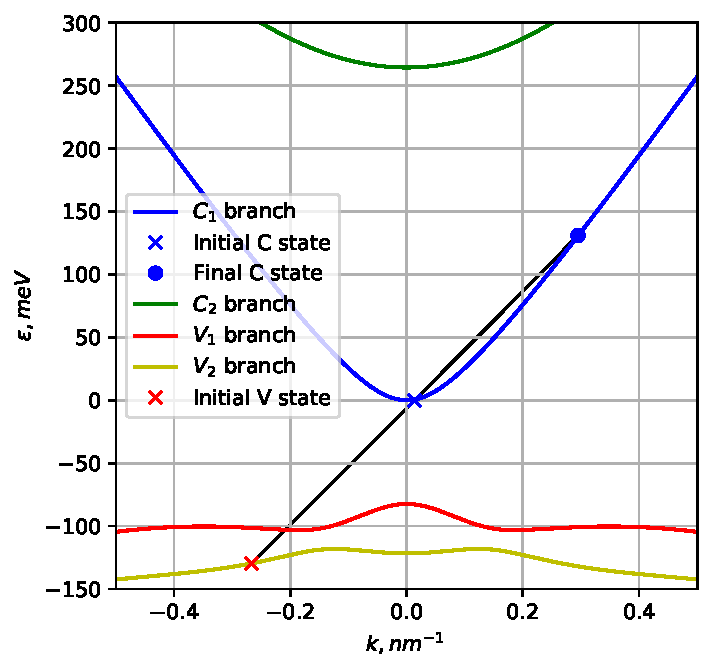
\includegraphics[width=\textwidth]{./images/add_pic.pdf}
        \end{center}
    \end{columns}
  \end{frame}

  \begin{frame}
    \frametitle{Сравнение с экспериментом $14~\mu m$}
    
    \begin{columns}
      \column{0.5\textwidth}
        При сопоставлении экспериментальных данных и теоретических расчетов порога была получена
        эмпирическая формула 
        связи критической для стимулированного излучения температуры и пороговой энергии: 
        \begin{equation*}
          T_{cr} \approx \varepsilon_{th} / 2;
        \end{equation*}
        Для её демонстрации была выбрана структура состава 
        $Hg_{0.903} Cd_{0.097}Te/Cd_{0.7} Hg_{0.3} Te$, имеющая 10 квантовых ям
        толщиной $7.4~nm$. 
        Было получено СИ в диапазоне $11-14~\mu m$ при температурах $18-85~K$. 
 
        Искомый процесс имеет тип CCHC и при $T=80~K$ соответственно
        $\varepsilon_g = 99~meV$, пороговая энергия $\varepsilon_{th} \approx 18.4~meV$, это соответствует 
        $T_{cr} \approx 100~K$.

      \column{0.5\textwidth}
        \begin{center}
          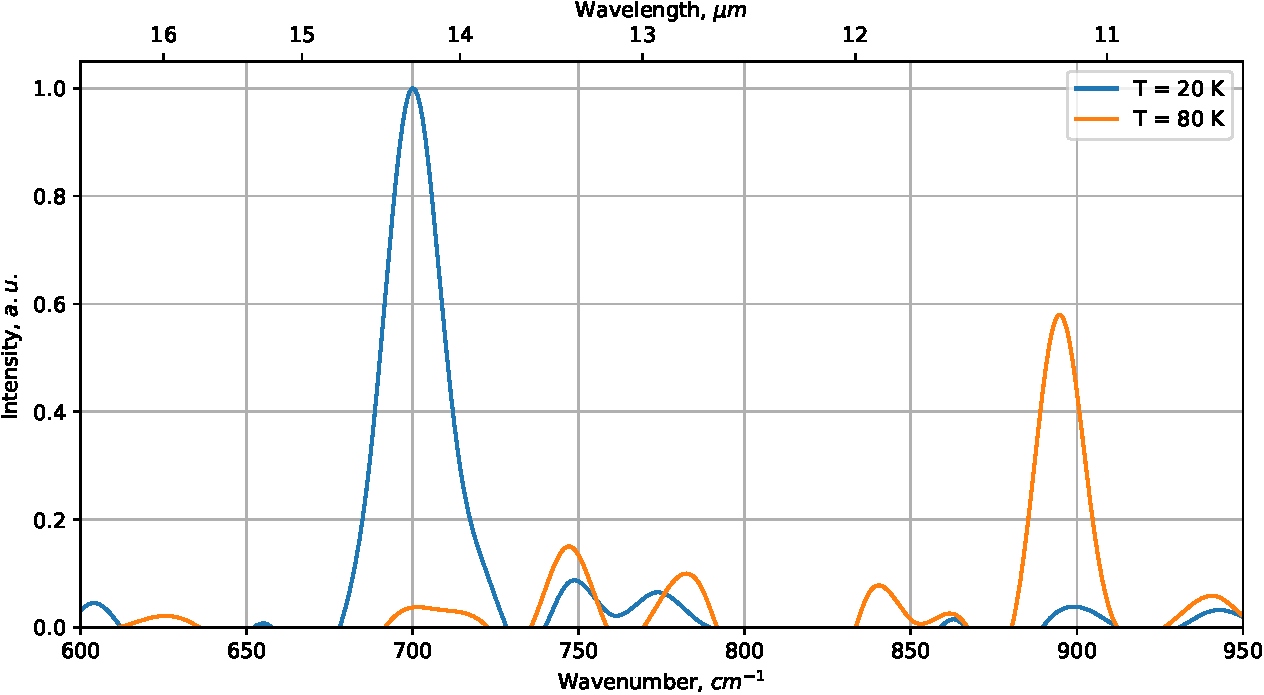
\includegraphics[width=0.8\textwidth]{./images/new_14um_spectre.pdf}
          
          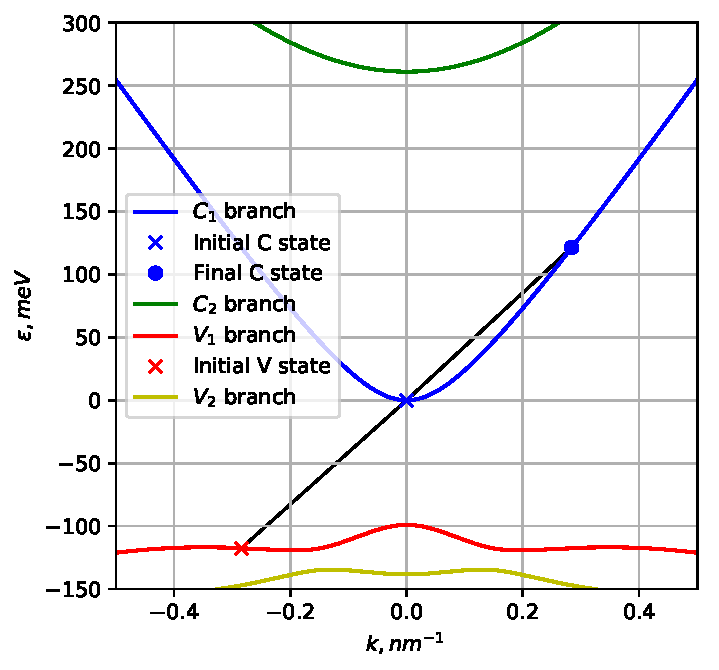
\includegraphics[width=0.9\textwidth]{./images/14u_impure_80K.pdf}
        \end{center}
    \end{columns}
  \end{frame}

  \begin{frame}
    \frametitle{Сравнение с экспериментом $18~\mu m$}
    
    \begin{columns}
      \column{0.5\textwidth}
        Аналогично для структуры, расчитанной на длину волны $18~\mu m$:
        $Hg_{0.9} Cd_{0.1}Te/Cd_{0.65} Hg_{0.35} Te$, имеющая 10 квантовых ям
        толщиной $8.7~nm$. 
        Было получено СИ в диапазоне $18~\mu m$ при температуре $50~K$. 
 
        Искомый процесс имеет тип CCHC и при $T=40~K$ соответственно
        $\varepsilon_g = 67~meV$, пороговая энергия $\varepsilon_{th} \approx 15~meV$, это соответствует 
        $T_{cr} \approx 80~K$.
        \vspace{3.5cm}

      \column{0.5\textwidth}
        \begin{center}
          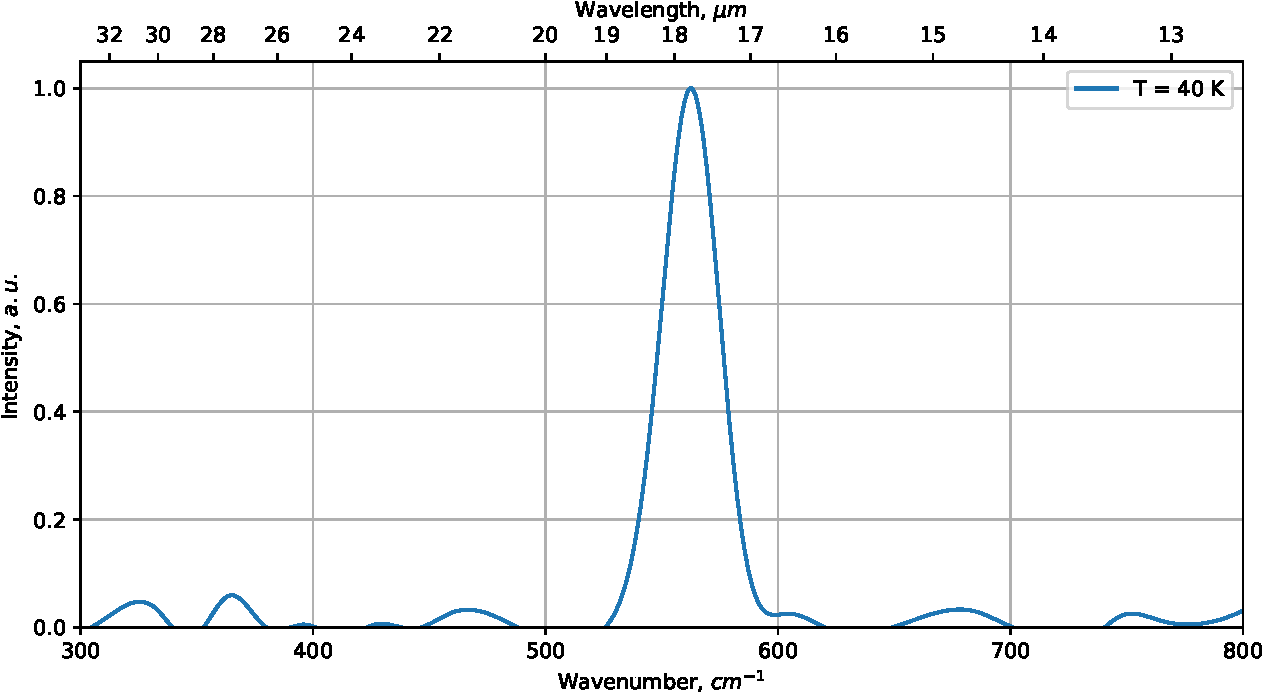
\includegraphics[width=0.8\textwidth]{./images/new_18um_spectre.pdf}
          
          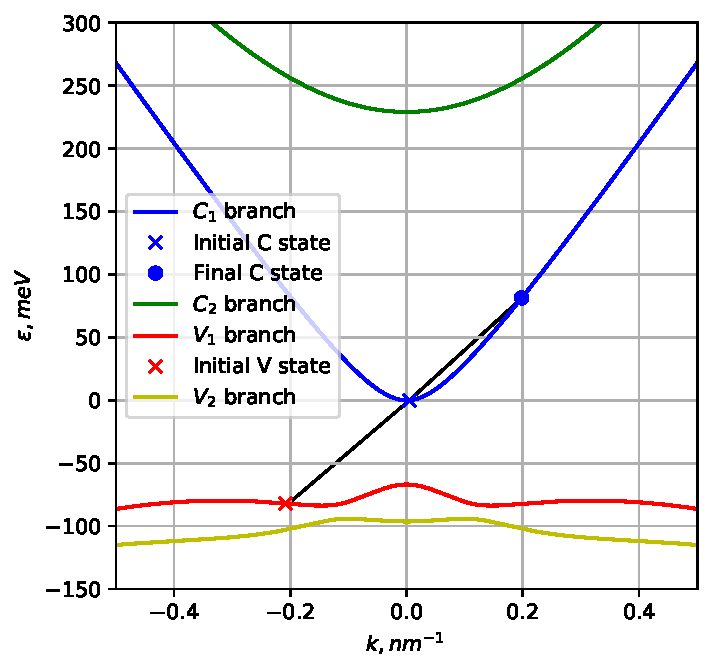
\includegraphics[width=0.9\textwidth]{./images/18u_impure_40K.pdf}
        \end{center}
    \end{columns}
  \end{frame}

  \begin{frame}
    \frametitle{Влияние наличия Cd внутри КЯ}

    \begin{columns}
      \column{0.5\textwidth}
        \begin{center}$\lambda\approx 14~\mu m$\end{center}

        \begin{figure}[t]
        \begin{center}
          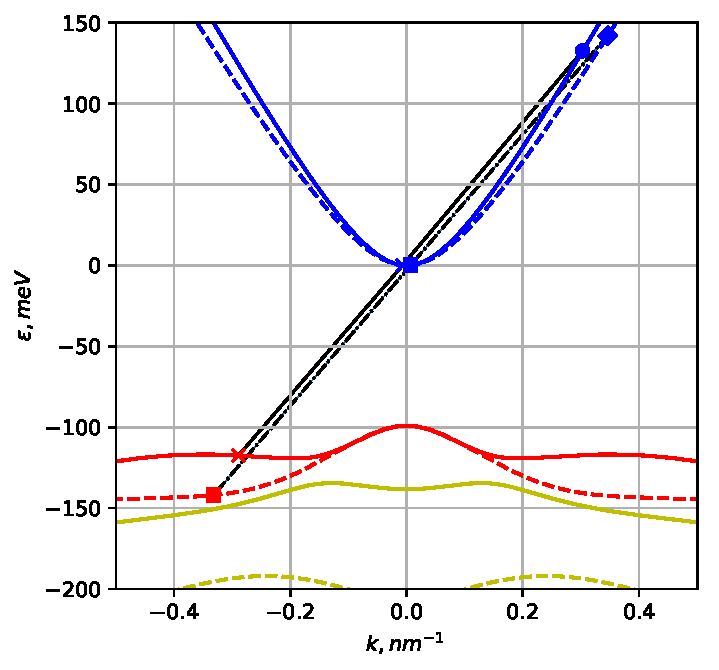
\includegraphics[width=0.8\textwidth]{./images/14um_p_vs_i.pdf}
        \end{center}
        \end{figure}

        \begin{figure}[b]
        \begin{center}
          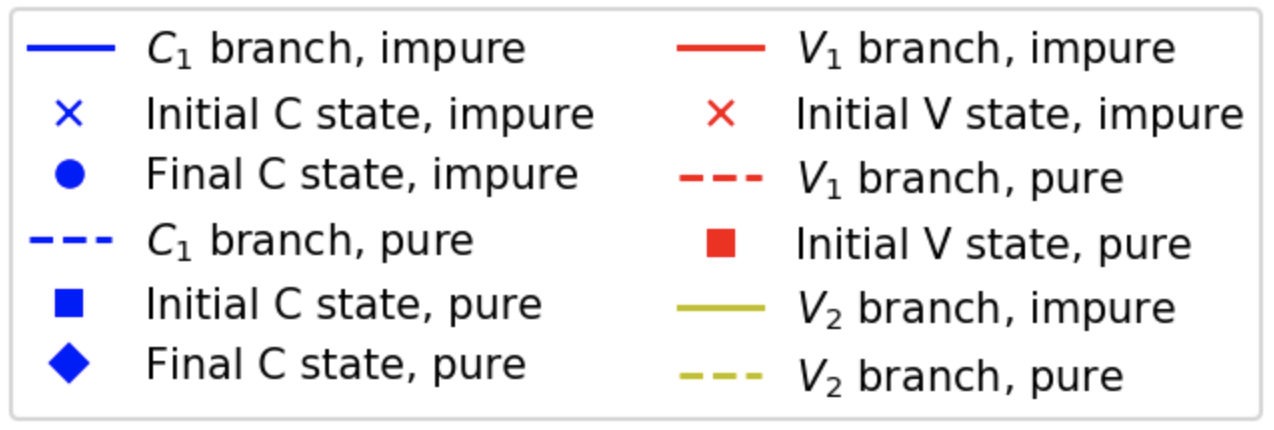
\includegraphics[width=0.8\textwidth]{./images/legend.png} 
        \end{center}
        \end{figure}

        \column{0.5\textwidth}

        \begin{center}$\lambda\approx 18~\mu m$\end{center}
        
        \begin{figure}[t]
        \begin{center}
          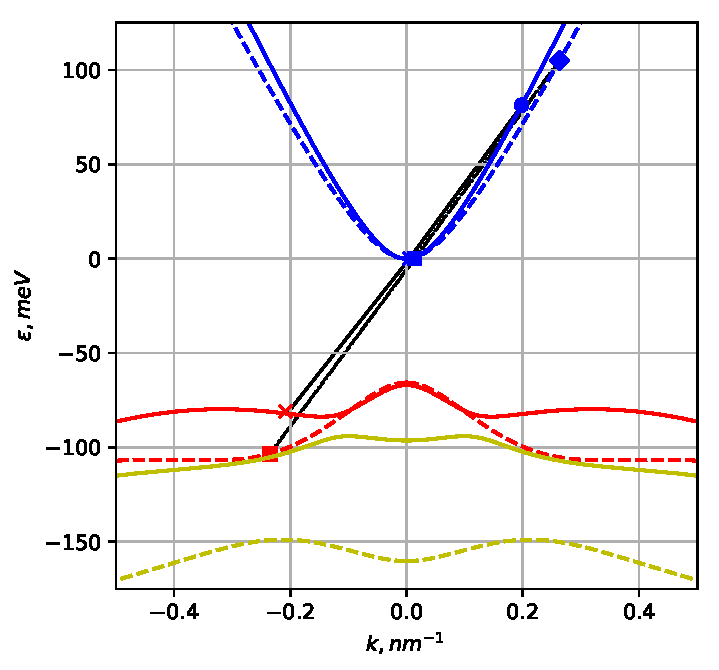
\includegraphics[width=0.8\textwidth]{./images/18um_p_vs_i.pdf}
        \end{center}
        \end{figure}

        \begin{figure}[b]
        Можно видеть разницу в пороговых энергиях для обоих структур.
          Она обусловлена наличием или отсутствием боковых максимумов.
          \vspace{0.223cm}
        \end{figure}
      \end{columns}
  \end{frame}

  \begin{frame}
    \frametitle{Порог оже-рекомбинации vs. состав барьера}

    \begin{center}
      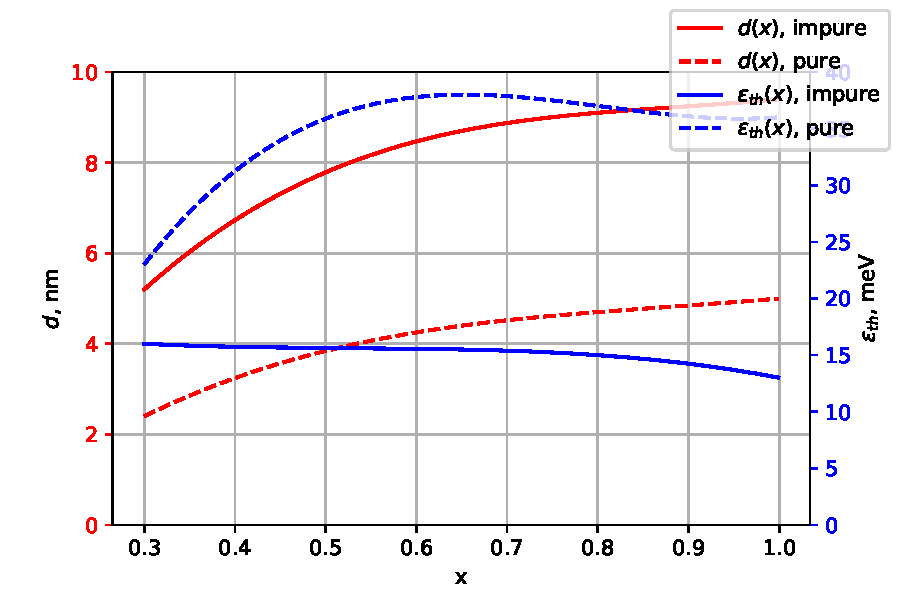
\includegraphics[width=0.8\textwidth]{./images/de_vs_x.pdf}
    \end{center}

    Как можно видеть, существует значительный максимум $\varepsilon_{th}$ при составе барьера
    Hg${}_{0.33}$Cd${}_{0.67}$Te. Аналогичные расчёты можно провести и для других структур.

  \end{frame}

  \begin{frame}
    \frametitle{Выводы и перспективы.}
    \begin{itemize}
      \item При сравнении экспериментально полученной критической температуры 
        с рассчитанным порогом оже-процессов наблюдается эмпирическая 
        закономерность $T_{cr} \approx \varepsilon_{th} / 2$.
      \item При фиксированной величине ширины запрещённой зоны, увеличение 
        концентрации кадмия в ямах ведёт к снижению порога.
      \item При фиксированной величине запрещённой зоны максимальная величина
        порога наблюдается при концентрации кадмия в барьерах  $0.55-0.65$.
    \end{itemize}
  \end{frame}

  \begin{frame}[t, allowframebreaks]
    \phantom{\cite{Rumyantsev:2019}, \cite{Kozlov:2019}, \cite{Utochkin:PTS:2019}, \cite{Rumyantsev:IOP:2018}, \cite{Rumyantsev:PTS:2018}}
    \frametitle{Литература}
    \bibliographystyle{plain}
    \bibliography{Bibliography}
  \end{frame}
\end{document}

